\documentclass[11pt]{article}
% Draft in a neutral layout; switch to the venue template once the target is fixed.
\usepackage[margin=1in]{geometry}
\usepackage[T1]{fontenc}
\usepackage{lmodern}
% Improve line breaking and keep text within the margins.
\usepackage{microtype}
\usepackage{amsmath,amssymb}
\usepackage{booktabs,multirow}
\usepackage{graphicx}
\usepackage[table]{xcolor}
\usepackage{tikz}
\usetikzlibrary{arrows.meta,positioning,fit,backgrounds,calc}
\usepackage[numbers,sort&compress]{natbib}
\usepackage{hyperref}
\hypersetup{pdfauthor={Chia Chen Yang}}
\usepackage[capitalise,noabbrev]{cleveref}

% Marks for the draft: what still needs evidence or checking.
\newcommand{\todo}[1]{\textcolor{red}{[TODO: #1]}}
\newcommand{\pending}[1]{\textcolor{orange}{[PENDING: #1]}}

\title{From a Sentence to an Annealer: A Local-LLM Agent System for\\
Real-World QUBO Optimization with Problem-Level Verification}
\author{Chia Chen Yang}
\date{Draft, \today}

\begin{document}
\maketitle

\begin{abstract}
Quadratic unconstrained binary optimization (QUBO) lets annealing hardware attack scheduling, routing, location
and many other combinatorial problems, but turning a real problem into a solved QUBO still takes an expert: the
problem must be pinned down, real data must be found and cleaned, the model must be written and checked, and
penalty weights and solver settings must be tuned on the hardware. Large language models
(LLMs) can draft QUBO formulations from natural language, but formulation correctness alone does not establish
that a workflow has acquired the intended data or delivered a usable decision.
We present a human-in-the-loop agent system that goes from a one-sentence problem description to a solution on
an annealer, built entirely on a locally served open model. The system clarifies the problem (with sourced web
lookup), lets the model choose and write the formulation under problem-independent structural checks, finds and
preprocesses public data through a typed sets-and-parameters interface, records provenance, and submits the QUBO to
interchangeable backends: simulated annealing, a GPU annealer, Fujitsu's Digital Annealer and D-Wave (direct QPU
and the Leap Hybrid service). The experiments reported here use simulated annealing, the GPU annealer and the
D-Wave Leap Hybrid service; the Digital Annealer rejected our submission at its monthly account limit. An outer
recovery loop checks data and model failures before any tuning, preserves model--data versions, and
distinguishes usable, limited and unavailable solutions. Penalty tuning is a secondary option for improving feasibility or quality against a baseline; the UI
starts with the default policy.
Separate checker roles compare prepared data with raw-table aggregates and model decisions with the confirmed
requirements. These checks provide repair evidence rather than correctness guarantees. Optional retrieval
supplies general modelling patterns. A person confirms the specification, approves data assumptions and reviews
the result; unresolved failures are returned with a diagnosis. A new real-data ablation protocol separates
pipeline structure, checking, repair and pattern retrieval; repeated evaluation under a frozen version remains
open.
We also show that the standard way of verifying LLM-written QUBOs is unreliable: in an audit of 33 failures of
an existing pipeline, at least 7 of 12 ``shape'' failures were caused by wrong LLM-written test cases rather than
wrong models, and one benchmark's reference answer contradicts itself. We propose problem-level verification,
which decodes every ground state and checks it with an independent checker anchored on the human-stated
optimum. Under it, the pipeline solves 70.3\% (69--72\%) of 100 benchmarks over three runs, while 27\% of the
benchmarks change outcome between identical runs. On a 12-category suite the local system produced a valid model
for all 36 runs, and the GPU annealer reached the exact optimum in 7 of the 9 categories with a known optimum.

\end{abstract}

\section{Introduction}
\label{sec:intro}

Quantum and quantum-inspired annealers, such as D-Wave's quantum processors, Fujitsu's Digital
Annealer~\citep{aramon2019digital} and GPU-based annealers, all accept the same input: a quadratic unconstrained
binary optimization (QUBO) problem. Many NP-hard problems have known QUBO formulations~\citep{lucas2014ising,
glover2019tutorial}, which makes QUBO an attractive common interface between real decision problems and new
hardware. In practice, however, a usable QUBO solution of a real problem requires a chain of expert work:
\begin{enumerate}
  \item pinning down what is actually being decided, under which rules (often laws or standards);
  \item finding real data, cleaning it and bringing it to a size the hardware can handle;
  \item writing a formulation that captures the confirmed objective and constraints;
  \item choosing penalty weights, encodings of inequality constraints and solver parameters, which strongly
        affect solution quality on hardware~\citep{verma2020penalty,ayodele2022penalty,pelofske2025comparing};
  \item explaining the result to the person who asked.
\end{enumerate}

Large language models (LLMs) have recently been used to automate step~3. QuantumQUBO
Agent~\citep{mondal2026quantumqubo} turns a natural-language description into a QUBO with a multi-agent pipeline
and verifies it by brute force on small test cases; related work does the same for mixed-integer
programming~\citep{ramamonjison2023nl4opt,ahmaditeshnizi2024optimus,xiao2024chainofexperts}. These systems stop at
the formulation, evaluate on toy-sized instances (in the QuantumQUBO benchmark, the median test case has five
binary variables), use large proprietary models, and list execution on hardware as future work.

Asking a frontier chat model the same question shows a different gap. It will write an objective and
constraints from one sentence and point to public datasets, but the rest of the work stays with the user: finding
and downloading the data, cleaning and joining it, running the solver, plotting and tuning. Our goal is to
automate exactly that remaining work, for real problems with real data, using a model that runs on a local GPU.

\paragraph{This paper.}
We build and study a human-in-the-loop system that takes a one-sentence problem (``place 20 EV chargers in
Taipei'', ``schedule 12 nurses for four weeks under Taiwan's Labor Standards Act'', ``plan a day of sightseeing in
Paris'') through data preparation, modelling, annealing and delivery. All agents run on one locally served open
model. People confirm the specification, approve data assumptions and review the result. The operational goal is
to complete this workflow or identify a concrete unresolved gap; it does not require a certified optimum for
every application. Poor results may trigger further solver search or a return to data and model repair,
depending on the evidence.

\paragraph{Research question.}
How can a locally served LLM, supported by specialized agent roles and executable feedback, turn a confirmed
request into a correctly prepared instance, a requirement-consistent model and a usable solution? Our design
separates these three obligations: feasibility of the generated model alone cannot establish the first two.
Multi-agent coordination and retrieval are mechanisms to evaluate, rather than benefits assumed from the
number of roles or the presence of a knowledge library.

\paragraph{Contributions.}
\begin{enumerate}
  \item \textbf{An end-to-end, local-LLM system from a sentence to an annealer (\cref{sec:system}).}
        Clarification with sourced web lookup; autonomous formulation under problem-independent structural
        checks; real-data acquisition and preprocessing with a tested toolkit and a provenance record;
        an encoding library with programmatic guardrails; one interface to four backend families (simulated
        annealing, a GPU annealer, the Fujitsu Digital Annealer and D-Wave QPU or Leap Hybrid), of which
        simulated annealing, the GPU annealer and Leap Hybrid were used in our experiments; and generated figures and
        explanations. Bounded recovery routes failures to data preparation, modelling or solving, retains
        versioned artifacts, and reports delivery status against a feasible conventional baseline.
  \item \textbf{A data model for ``real problems'' (\cref{sec:setting}).} Each input of a model is either
        public data (found, never invented), a user setting (asked, with defaults) or private data (uploaded,
        or explicitly marked mock data). This makes ``uses real data'' a checkable property of a run instead of
        a claim, and it decides what the system automates and what it asks. The current implementation declares
        entity sets, indexed parameters, units and derivations explicitly; a separate Data Checker can compare
        counts and totals with computations on the raw tables.
  \item \textbf{Problem-level verification of LLM-written QUBOs (\cref{sec:verification}).} We show that
        bitstring-based verification with LLM-derived reference solutions misjudges models in both directions,
        and that the reference answers of a public benchmark can themselves be inconsistent. We replace it with
        a check that decodes every ground state and evaluates it with an independent checker anchored on the
        human-stated optimum, and we quantify run-to-run instability that single-run evaluations hide. For
        larger real-data instances, a separate Requirement Checker samples decisions against the confirmed
        request and checks delivered decisions; this sampled check does not certify all model states.
  \item \textbf{Failure modes of a small local model as an autonomous modeller, and mechanisms that address
        them (\cref{sec:system,sec:experiments}).} We document recurring failures (empty objectives, constraint
        penalties folded into the objective, silent over-simplification into a sortable problem, dropped hard
        constraints, exhausted reasoning budgets, prompt overflow on large models) and the generic mechanisms
        that address them: task splitting, repair instead of rewrite, constraint families and prompt budgets.
        The current system also implements bounded data-to-model repair and optional retrieval of general
        modelling patterns; their end-to-end effects require the ablations in \cref{sec:autonomousprotocol}.
  \item \textbf{An empirical characterization (\cref{sec:experiments}).} A 12-category end-to-end suite, the
        scaling of a GPU annealer on routing up to 3{,}600 variables, and a budget-matched comparison of
        LLM-driven tuning with rule-based, random and Bayesian-optimization baselines, which shows that penalty
        tuning benefits depend on the instance and backend (\cref{sec:penaltysummary}; details in \cref{app:details}).
\end{enumerate}

The current autonomous acceptance suite targets Taipei EV-charger coverage, a YouBike inspection tour and AED
inspection grouping. Its evaluation judge is separate from the runtime agents. Development runs have exposed
both successful deliveries and upstream failures; they are not pooled into a success rate because code and
prompts changed between runs. The earlier synthetic suite and specified-source pilots remain separate evidence
(\cref{sec:autonomousprotocol,sec:limitations}).

\section{Related Work}
\label{sec:related}

\paragraph{LLMs for optimization modelling.}
NL4Opt~\citep{ramamonjison2023nl4opt} framed the translation of natural-language problem descriptions into linear
programs as a benchmark. OptiMUS~\citep{ahmaditeshnizi2024optimus} and Chain-of-Experts~\citep{xiao2024chainofexperts}
use agents to formulate and solve (mixed-integer) linear programs with classical solvers. For QUBO, QuantumQUBO
Agent~\citep{mondal2026quantumqubo} decomposes the task into planner, formulator, judge, coder and debugger agents
and verifies the generated QUBO by enumerating all bitstrings of small test cases;
LLM-QUBO~\citep{llmqubo2025} also goes from language to a solved QUBO. All of these evaluate whether a formulation
is correct; none acquires real data, and none adapts the formulation or the solver to what the hardware returns.
We build on QuantumQUBO Agent's benchmark and pipeline, show that its verification protocol is unreliable
(\cref{sec:verification}), and extend the scope to the whole path from a sentence to a hardware solution.

\paragraph{QUBO formulation and penalty weights.}
Standard formulations of NP-hard problems are collected by Lucas~\citep{lucas2014ising} and Glover et
al.~\citep{glover2019tutorial}. Constraint penalties must be large enough to keep infeasible states out of the
ground state but small enough to preserve precision and the energy landscape; bounds and heuristics for them are
studied by Verma and Lewis~\citep{verma2020penalty}, adaptive weights on the Digital Annealer by Ayodele et
al.~\citep{ayodele2022penalty}, and learned or black-box tuning of penalties in recent
work~\citep{penaltyml2025bisection,formulationautotuning2026}. Inequalities can be encoded with slack variables or
by unbalanced penalization~\citep{montanez2024unbalanced}, which avoids slack variables but is approximate. Our
encoding library implements these choices, labels approximate encodings, and checks tuning actions against
encoding-specific heuristics. The original constraints and objective remain the basis for evaluating results.

\paragraph{Reusable penalty-search software.}
PyQUBO provides placeholders for changing coefficients without recompiling an expression and labelled
constraint diagnostics~\citep{pyquboDocs}. QHyper treats penalty weights as hyperparameters and supports grid
and cross-entropy search~\citep{qhyperDocs}. Kaiwu's penalty-method solver exposes feasible-result stopping
and checkpoint mechanisms~\citep{kaiwuDocs}. We directly use PyQUBO and Optuna~\citep{akiba2019optuna}; our
local grid, cross-entropy and sequential policies adapt the search and control designs of QHyper and Kaiwu
to the existing backend interface. We do not call the latter two SDKs. The system-level focus is routing
execution failures to the appropriate data, model or solver stage and retaining a deliverable result; we do
not claim a new penalty-search algorithm.

\paragraph{Annealing hardware and parameter tuning.}
D-Wave annealers require minor embedding and are sensitive to chain strength and annealing
time~\citep{pelofske2025comparing}; the Digital Annealer~\citep{aramon2019digital} and GPU annealers accept dense
QUBOs but expose different parameters and precision limits. Benchmarks such as QOBLIB~\citep{koch2025qoblib}
provide hard instances with known optima. Black-box hyperparameter optimizers such as
Optuna~\citep{akiba2019optuna} are the natural non-LLM baseline for tuning, and we use them as such.

\paragraph{Closest work: LLM agents with hardware in the loop.}
Wang and Lu~\citep{wang2026cim} use LLM agents to iterate constraint weights on a coherent Ising machine. Their
work is the closest to our tuning loop; it targets a single backend and, to our knowledge from the abstract,
reports no budget-matched baselines. Our system spans four backends with one interface, keeps tuning
subject to programmatic guardrails, compares against rule-based, random and Bayesian
optimization at equal solver budgets, and adds the front end (clarification, modelling, real data) that makes the
loop applicable to problems stated in plain language.

\paragraph{Agents, tools and local models.}
Our agents follow the reason-and-act pattern~\citep{yao2023react} in a deliberately constrained form: the language
model decides, while deterministic code executes, checks and enforces budgets. All agents run on a locally served
open model~\citep{qwen3report2025} through vLLM~\citep{kwon2023vllm}; the system can route any single role to a
stronger remote model when needed. Real data comes from open-data platforms and
OpenStreetMap~\citep{osm}, with road distances from OSRM~\citep{luxen2011osrm}.

\section{Problem Setting and Design Principles}
\label{sec:setting}

\paragraph{Task.}
The input is a problem described in plain language, possibly in one sentence. The output is (i)~a specification
confirmed by the user, (ii)~the data used, with provenance, (iii)~a validated binary optimization model and its
QUBO, (iv)~a feasible solution evaluated against a conventional baseline where available,
and (v)~a figure and a plain-language explanation of the result and its assumptions. Delivery identifies whether
the solution came from an annealer or the baseline. If no usable solution is available, the output states the
failed stage, attempted repairs and missing information rather than reporting success because execution ended.

\paragraph{Operational success and model verification.}
The workflow seeks a feasible, interpretable result within a bounded resource budget. A known optimum is
optional; a feasible baseline supplies a quality comparison when no optimum is available. This operational goal
is distinct from the benchmark protocol in \cref{sec:verification}, which uses small instances with stated
optima to test whether a generated formulation is correct.

\paragraph{Three classes of model inputs.}
``Real problems need real data'' is too coarse to act on: some inputs are facts about the world, some are
preferences of the decision maker, and some are private. Every input field of a model is assigned to one class,
and the class decides what the system does (\cref{tab:dataclasses}). A run counts as a \emph{real-data run} only if
every class-A field comes from a cited source; fields filled by the model's own estimates are reported, never
hidden.

\begin{table}[t]
\centering
\caption{Classes of model inputs and the system's behaviour for each.}
\label{tab:dataclasses}
\small
\begin{tabular}{@{}lp{4.2cm}p{6.3cm}@{}}
\toprule
Class & Examples & System behaviour \\
\midrule
A: public data & locations, population, existing facilities, road distances, laws, price histories &
  searched, downloaded and preprocessed; every value traceable to a source; if not found, the gap is reported and
  never filled silently \\
B: user setting & visit durations, number of sites to open, budget, objective weights &
  asked with sensible defaults the user can change; not ``data'' and not searched for \\
C: private data & staff rosters, availability, internal costs and orders &
  uploaded by the user; otherwise mock data, explicitly labelled as such in every output \\
\bottomrule
\end{tabular}
\end{table}

\paragraph{Design principles.}
\begin{enumerate}
  \item \emph{The model decides, code executes and checks.} Agents propose specifications, formulations, data
        mappings and tuning actions as structured output; deterministic code validates, runs and enforces budgets.
        Control flow is fixed, which keeps runs reproducible and every agent replaceable for ablations.
  \item \emph{People confirm the specification, data assumptions and result.} The system can search and prepare
        alternative data automatically, but unresolved substitutions or changes to requirements return to the
        user. Choosing which dataset represents ``demand'' remains a modelling decision.
  \item \emph{Local first.} Agent inference uses one locally served open model, avoiding a hosted-LLM dependency in the
        reported configuration. Local inference still consumes compute, and cloud annealers receive the
        submitted optimization instance; local serving alone does not guarantee that all data stays on the
        machine. Individual roles can be routed to another model or provider by configuration.
  \item \emph{Problem-independent mechanisms only.} When the model fails, we add checks that say \emph{what} is
        wrong (an empty objective, a dropped hard constraint) rather than embedding a complete case-specific formulation in the prompt. Optional retrieval supplies
        reusable modelling patterns, while the LLM still writes the instance-specific formulation.
        Case-specific acceptance judges are evaluation artifacts, not inputs to the runtime agents; earlier
        specified-source pilots used manually prepared specifications and checks.
  \item \emph{Check tuning against the original problem.} Code enforces penalty heuristics, encoding-specific
        checks, solver ranges and call budgets. Exact encodings are distinguished from approximate ones, and
        feasibility and solution quality are evaluated on the original constraints and objective. A
        single-flip penalty floor is not a certificate that a large QUBO preserves every global optimum.
\end{enumerate}

\section{System}
\label{sec:system}

\Cref{fig:arch} shows the forward pipeline. Each stage combines proposal generation with deterministic checks;
the recovery controller can return a failed run to an earlier stage.

\begin{figure}[t]
\centering
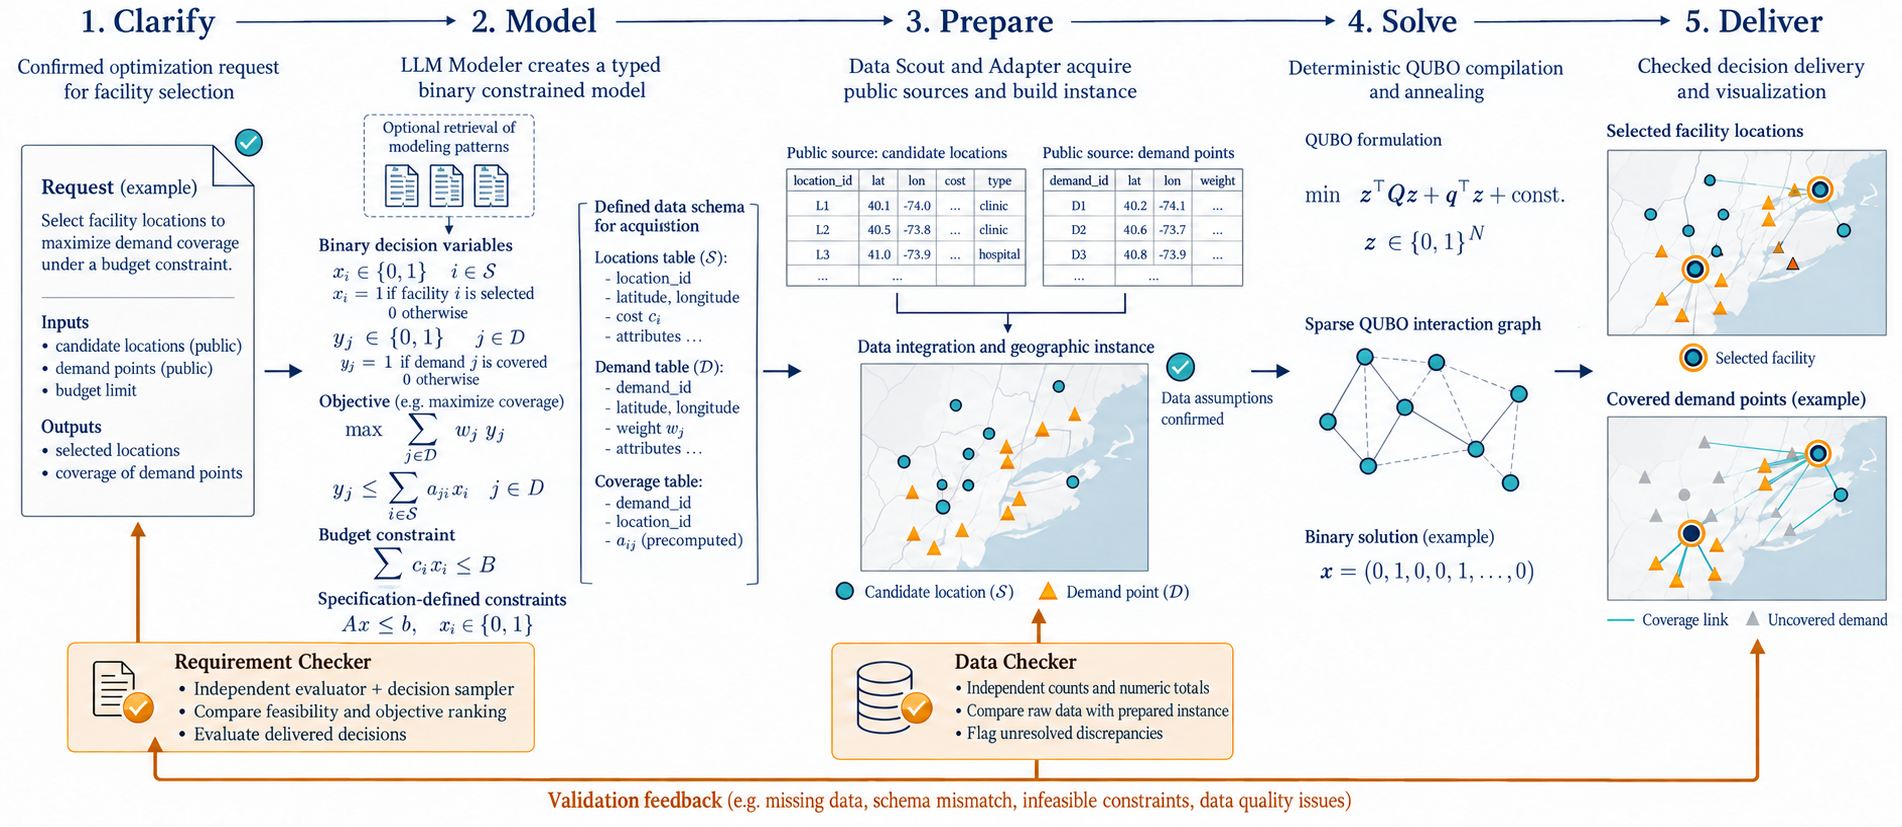
\includegraphics[width=\linewidth]{figures/skill/workflow-illustrated.png}
\caption{Illustrative end-to-end facility-selection workflow. A confirmed request becomes a typed binary
model and schema, a prepared public-data instance, a QUBO and a checked decision. Coverage variables prevent
double-counting; QUBO variables include decision and encoding auxiliaries. Checker evidence supports bounded
repairs, not a guarantee of correctness. Tables, coordinates, maps and bit assignments are schematic examples.}
\label{fig:arch}
\end{figure}

\subsection{Clarification}
The Clarification Agent drafts a specification (decision variables, objectives, hard and soft constraints, data
needs, a size estimate against the target backend) and asks at most five questions per round, each with options
and a suggested default; everything else it decides itself and records as an assumption that the user accepts or
corrects at confirmation. When the specification depends on external facts (laws, standards) it proposes up to
three search queries; code runs them, fetches the pages (including government sites and PDFs) and extracts the
passages relevant to the query, and the agent drafts again with the findings. Every claim taken from the web must
cite a page that was actually fetched: garbled URLs are corrected to the nearest fetched page and anything else is
marked unverified. Findings are stored with the session, so a rerun does not search again.

\subsection{Modeling}
The Modeling Agent writes a Python module: a data schema, a synthetic data generator, a builder that returns a
typed model over binary variables (linear and quadratic objective terms; linear, exclusion and implication
constraints), and a function that describes a solution. It also states its own modelling choice (e.g.\ an exact
formulation or an approximation that fits the target hardware). Code validates the module on a small instance by
brute force and with problem-independent checks, each of which was added after observing the failure it detects:
\begin{itemize}
  \item the data survives a JSON round trip (the model is later fed stored data);
  \item the objective is not empty;
  \item no hard constraint's squared penalty is folded into the objective (detected as uniform couplings over the
        constraint's variables);
  \item hard constraints of the specification are not all missing from the model;
  \item the model is not solvable by sorting, i.e.\ it does not consist of a linear objective with
        non-overlapping ``choose $k$'' constraints, unless the agent declares and justifies it;
  \item the small instance is feasible, with a hint when a parameter is not scaled to the instance size.
\end{itemize}
Retries show the agent its previous module and the errors and ask for a repair rather than a rewrite. Drawing is
split into a separate short task: a Visualizer writes a function that returns a figure \emph{specification} in one
of five fixed formats (map, schedule, routes, graph, selection), which code validates and renders.

\subsection{Data acquisition and preprocessing}
A Data Scout turns the model's data schema into searches on open-data platforms and OpenStreetMap, and screens
candidates for relevance and readability. Connectors support CKAN, Socrata, Opendatasoft, ArcGIS Hub and the
European data portal; supported WFS layers are requested as JSON in WGS84. These connectors use links returned
by catalog APIs or fetched source pages. Their implementation does not establish reliable coverage of every
portal or data format. The user can select sources manually, or a bounded acquisition
controller tries existing readable tables and then alternative sources. Download and conversion failures are
recorded; a retry receives the preceding errors rather than repeating the same request blindly. Unresolved
data gaps and assumptions are surfaced for confirmation. A Data Adapter maps the tables to
the model's schema. It never reads raw data: it sees bounded profiles of each table (columns, types, ranges,
missing values, a few rows) and writes code that runs on the full tables, preferably by calling a tested
preprocessing toolkit for situations that recur in public data: encodings (Big5, UTF-8 with BOM), Shapefiles and
GeoJSON, total and subtotal rows, rows split by category, stacked periods, mixed administrative levels, ROC
calendar dates, numbers stored as text, coordinate systems (via EPSG codes), variant characters in place names,
geocoding with explicit precision levels, road distance and time matrices, and size reduction by weighted
clustering. Every step is written to a provenance record (sources, licences, row counts, match rates) that the
user can inspect before approving data assumptions. Unknown licences remain marked as unknown. The adapter's
output is checked on the full data against the declared interface and example input.

\paragraph{Typed data interface and administrative joins.}
The current \texttt{DATA\_SCHEMA} separates entity sets from parameters indexed by those sets. It declares
source class, type, unit, derivation and, where available, period, geography and granularity. Checks reject
unknown fields, duplicate entity IDs, incompatible dense-array shapes, invalid sparse indices and invalid
numeric values. Canonical spatial inputs use WGS84 latitude and longitude, and distance parameters use metres.
Derived fields can require specific toolkit calls. For mixed administrative levels, the toolkit can propagate a
parent district before filtering village rows, then join on district and village together; duplicate keys and
unmatched rows are reported. These checks address common loss and misalignment mechanisms, but declared units
and correctly shaped arrays can still encode the wrong interpretation.

\paragraph{Independent data computation.}
When enabled, a Data Checker receives the confirmed request, schema and raw-table profiles, but not the Adapter
code. It writes a separate computation of expected entity counts and numeric totals. Code compares these with
the prepared instance, using a 0.5\% total tolerance with a unit-scale floor. Counts are skipped for sets declared
reducible. Disagreements trigger bounded Adapter feedback; a remaining disagreement is marked for review.
Checker-generation failures are recorded. This optional mechanism is enabled in the checker arms of the batch
protocol, not universally in every acquisition call. Aggregate agreement cannot detect every wrong join,
per-entity permutation or shared misunderstanding by the two LLM roles.

\paragraph{Acquisition safeguards.}
Several problem-independent rules come from failures in development runs. Candidates are screened by a
preview of their first bytes (column names and a first record) as well as by title, and raw record tables are
preferred over reports and documentation. A candidate is relevant if it supplies at least one required item, since
sources are joined later; boundary maps count as sources of coordinates. When one dataset holds several period
files, code keeps only the latest; when the request names a publisher, that publisher's data take precedence over
crowd-sourced points. The loader extracts record lists nested in JSON responses, recognizes web pages saved
under data names, tolerates isolated malformed rows (and reports them), skips title lines above a header, and
streams large files to disk. Coordinates stored as text are inspected for projected systems, and $(0,0)$
coordinates are rejected as missing values. When a join on names finds duplicate keys and both tables carry a
parent level, the join adds that level itself; otherwise the flag explains how to recover the parent level.

\paragraph{Requirement Checker and decision identities.}
\Cref{fig:verificationlayers} separates the runtime checker roles from the external evaluation judge.
A separate Checker generates an evaluator and decision sampler from the confirmed specification and data
schema without seeing the model formulation. Model variables carry \texttt{variable\_keys} that identify their
underlying decisions independently of bit positions. Before solving, sampled decisions are evaluated both by
the Checker and by the model with decision variables fixed; a time-limited MILP optimizes remaining helper
variables where supported. Tests compare feasibility, objective ranking and rejection of perturbed decisions.
After solving, the Checker evaluates the delivered decisions. Timeouts and unsupported helper interactions
remain inconclusive, and so do sampled decisions that have no model variable (a model may fix some decisions to
break symmetry, e.g.\ the first stop of a closed tour). The Checker computes distances with the same tested
toolkit as the Adapter and must not require what the specification leaves free. A disagreement supplies repair evidence; because the Checker is also LLM-generated,
agreement is not a proof of semantic correctness. The acceptance judge in \cref{sec:autonomousprotocol} is
separate from this runtime role.

\begin{figure}[tbp]
\centering
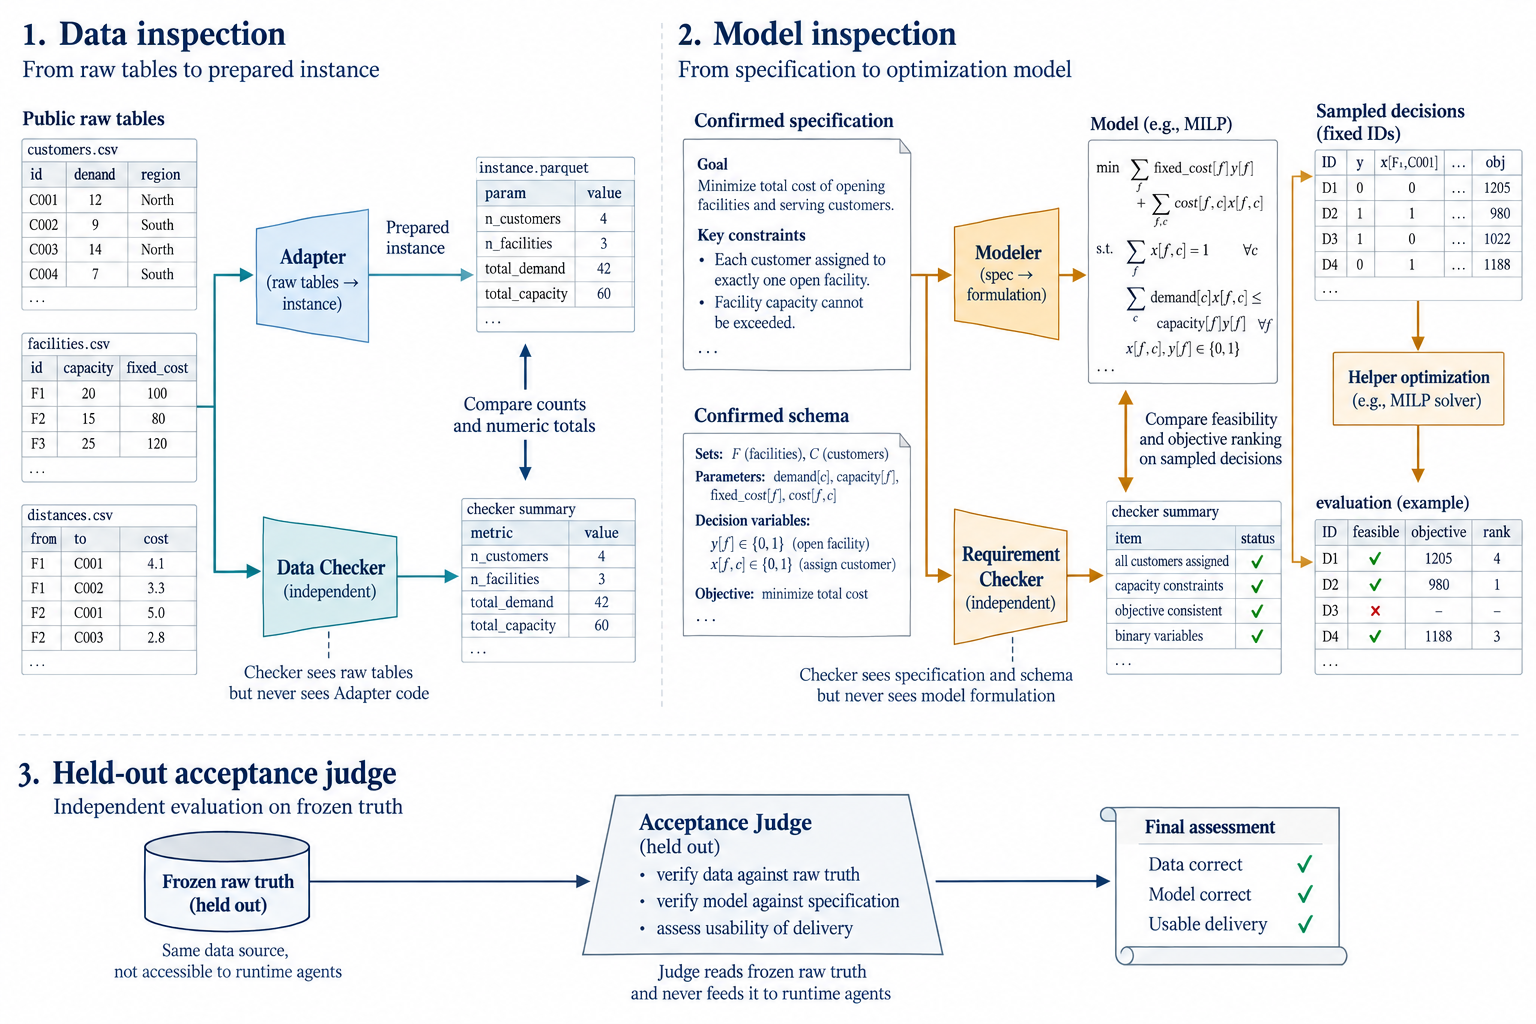
\includegraphics[width=\linewidth]{figures/skill/verification-reference.png}
\caption{Illustrative data inspection, requirement inspection and external acceptance judging. Tables,
formulations, evaluation values and check marks are schematic examples, not experimental results.
Agents receive bounded raw-table profiles and write code that operates on full tables; the Requirement
Checker does not see the formulation. Helper optimization is used where supported. Checker agreement is
evidence rather than a correctness guarantee; held-out judge truth is not supplied to runtime agents.}
\label{fig:verificationlayers}
\end{figure}


\paragraph{Optional retrieval of modelling patterns.}
The Modeling Agent can select up to three general patterns by title from a local knowledge library and receive
their text in its modelling prompt. Repairs reuse the selected pattern IDs. This is a bounded retrieval step,
not a pretrained change to the LLM or an embedding-based search service. The pattern-retrieval arm tests its
incremental effect; the earlier tuning-knowledge experiment addresses a different stage.

\subsection{Encodings, guardrails and the tuning loop}
Constraints are compiled to QUBO penalties through an encoding library (squared penalties for equalities, binary
or unary slack and unbalanced penalization~\citep{montanez2024unbalanced} for inequalities, pairwise penalties for
exclusions and implications), each verified in both directions on small cases. A tuning loop proposes penalty
weights, encodings and solver parameters, runs the backend, extracts backend-independent feedback (feasibility,
violation rates per constraint, objective, gap, energy spread, backend-specific signals such as chain breaks) and
proposes the next configuration. Guardrails reject weights below the single-flip lower bound for exact
encodings~\citep{verma2020penalty}, unbalanced penalties whose reward on feasible points exceeds the objective's
range, out-of-range solver parameters and anything beyond the hardware budget. On large models agents see
constraint \emph{families} (names with numbers abstracted) instead of individual constraints, which bounds prompt
size by the number of constraint kinds rather than by the instance size. The single-flip floor is a heuristic
guardrail, not a general proof of global-optimum preservation. Results are ranked by original-problem
feasibility and objective; QUBO energy is diagnostic because changing penalties changes its meaning.

\paragraph{Parameterized compilation and diagnostics.}
For each encoding combination, the compiler assembles the objective and unit-weight penalties in PyQUBO and
compiles once~\citep{pyquboDocs}. Subsequent rounds substitute named penalty placeholders. Explicit variable
labels preserve the original decision and slack indices. Labelled penalties help diagnose a selected sample,
but do not replace original-constraint checks: a feasible decision may have incorrectly filled slack variables
and hence a nonzero encoded penalty. Approximate unbalanced penalties are excluded from zero-penalty
constraint diagnostics.

\paragraph{Penalty-only search policies.}
The UI selects \texttt{default} initially; penalty-search policies remain explicit alternatives.
Alongside the existing agent, rule, random and joint Optuna policies, four policies vary penalties while
keeping solver effort at its capped defaults. Optuna TPE uses two startup trials; its score assigns every
feasible result a higher value than an infeasible result, then reflects the original objective. Grid search
enumerates a bounded logarithmic grid lazily. Cross-entropy search updates a log-weight distribution from
elite rounds ranked by original-problem quality, with a variance floor and bounded sampling attempts.
A sequential controller doubles penalties of violated constraints up to a configured ceiling. The grid and
cross-entropy designs draw on QHyper~\citep{qhyperDocs}, while sequential control, feasible-round stopping
and checkpointing draw on Kaiwu~\citep{kaiwuDocs}; these are local adaptations, not SDK calls.
All policies share the backend interface, guardrails and solver-call budget.

\paragraph{Stopping and checkpoint recovery.}
The controller can optionally stop after a configured number of rounds containing a feasible solution; this
condition is disabled by default and does not certify quality. After each completed round it saves the typed
model, settings, feedback, feasible penalty configurations and cumulative call count. The four penalty-only
policies reconstruct their search state from this history. Resume checks the model, backend, policy, seeds and
settings, while allowing an increase in the total call budget. A pending marker is written before submission;
if an interruption leaves a call unresolved, automatic resubmission is refused until the backend record is
inspected. This does not provide an exactly-once transaction at an external solver.

\subsection{Recovery across data, modelling and solving}
\label{sec:recovery}
\Cref{fig:recoveryroutes} summarizes the evidence used to route a run through checking, repair and delivery.
Before annealing, the controller checks basic data and constraint consistency and runs a time-limited HiGHS
feasibility check. Proven infeasibility is reported without an annealer call; timeout remains unknown and
does not imply that the problem has no solution. A feasible conventional solution supplies a quality baseline.
For quadratic objectives, the baseline combines a feasible point with bounded local improvement; it is not
labelled an optimum. Only a certified optimum of the linear model is used as an exact reference.

Before solving, a bounded repair callback can regenerate the model when acquisition reports a schema mismatch,
then rerun preparation against the new interface. Source-download failures and arbitrary Adapter exceptions do
not automatically imply a modelling fault. Workflow callbacks can subsequently use data or requirement-check
evidence to propose a revised Adapter or model.

Solver failure alone does not justify changing the model. Evidence of a formulation error can route the run
back to modelling; data mismatches route it to preparation, and unresolved resource shortfalls return a
diagnosis to the user. Repairs are bounded and share the remaining solver-call budget. A replacement is
validated before becoming active. A requirement map checks coverage of every confirmed hard requirement; a requirement guaranteed by the variable
design itself (e.g.\ a single closed tour under position encoding) is mapped with a stated justification and is
still tested by the Requirement Checker and the judge. Clarification records what must hold, not modelling
techniques.
Code repairs are compared on the same original data: changes to existing constraint formulas, bounds or
objective coefficients require confirmation. Fixed user inputs are protected against data-level changes.
Explicit data contracts check declared units, periods, scope, granularity and source correspondence;
unknown metadata remains a review item. These checks cannot prove that a repair preserves the natural-language
specification or that declared data semantics are true.

Model code, data and provenance are stored together in immutable versions with an atomic active pointer.
A durable task record states the current stage and next action. Prepared-data caches require matching code,
specification, notes and file hashes; the UI can resume supported solver checkpoints.
Generated model and adapter code runs in separate processes with timeouts, limiting hangs and crashes; this
is process isolation rather than a security sandbox. Results are tied to the version that produced them.
Delivery distinguishes usable solutions, solutions with limited quality, and absence of a usable solution.
If the annealer produces no feasible solution or trails the validated baseline beyond the configured
tolerance, the baseline can be delivered with its source stated. A Checker objection after solving triggers a
model repair only while solver calls remain to solve the repaired version; otherwise the solution is delivered
with the objection as a warning, and a repaired version left unsolved falls back to the earlier version's
annealer result. Figure or explanation failure does not
discard the saved solution.

\begin{figure}[tbp]
\centering
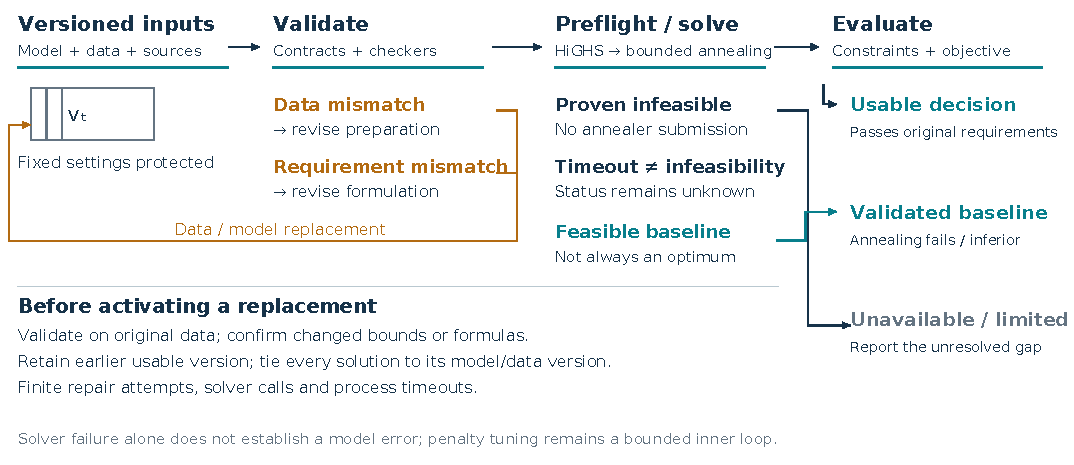
\includegraphics[width=\linewidth]{figures/skill/recovery-routes.pdf}
\caption{Evidence routes failures to the relevant stage. A repaired version must pass checks before activation.
Proven infeasibility avoids an annealer submission; a timed-out preflight does not prove infeasibility.
A validated baseline may be delivered when annealing fails or trails it. Repairs and solver calls are bounded.}
\label{fig:recoveryroutes}
\end{figure}


\subsection{Backends and serving}
The same QUBO can be submitted to simulated annealing (dwave-samplers), a GPU annealer (Compal GPU Annealer 2.0,
cloud service), the Fujitsu Digital Annealer v3c~\citep{aramon2019digital} and D-Wave (Advantage QPU or the Leap
Hybrid BQM service), with energies recomputed locally so results are comparable across backends. Our experiments
use simulated annealing, the GPU annealer and Leap Hybrid; a Digital Annealer submission was rejected at the
account's monthly usage limit, and no direct-QPU results are reported. All agents use Qwen3.6-35B-A3B (FP8)~\citep{qwen3report2025}
served by vLLM~\citep{kwon2023vllm} on NVIDIA L40S GPUs; each call has a reasoning budget, and an answer that
exhausts it is retried once without reasoning.

\section{Problem-Level Verification of LLM-Written QUBOs}
\label{sec:verification}

\subsection{The bitstring protocol and its failure modes}
QuantumQUBO Agent~\citep{mondal2026quantumqubo} verifies a generated QUBO on small test cases: an LLM converts each
human-written test case of a benchmark (instance, optimal value, an optimal solution in words) into a JSON case
with a variable count $n$ and the optimal \emph{bitstrings} in the formulation's own variable layout; code then
enumerates all $2^n$ bitstrings and accepts the QUBO if its minimizers overlap with the reference bitstrings.
The LLM that writes the reference bitstrings must therefore count the variables of the formulation, apply its
index map, and fill in auxiliary and slack variables correctly, all without executing anything.

We audited all 33 failures of the pipeline in a run with a local model (67/100 successes) by re-running the final
code of each failed benchmark on its test cases and inspecting the cases. Twelve failures were shape mismatches
between the generated $Q$ and the case's $n$. Comparing each case with the formulation's own variable map, the
\emph{test case} was wrong in at least 7 of the 12 (e.g.\ $n=9$ written for a model whose map gives
$4+5+5=14$ variables, while the code correctly built 14), the code was wrong in 2, and 3 were undetermined. Six
further failures were format mismatches between the case's instance and what the code read, and eleven were
argmin mismatches. One benchmark, quadratic assignment, is internally inconsistent: its stated optimal assignment
costs 20 while its stated optimum is 12 (the optimum of 12 is attained by a different assignment), so a correct
model fails whenever the reference bitstring follows the stated assignment.

\subsection{Problem-level verification}
We verify what a QUBO's ground states \emph{mean} instead of how they are laid out.
\begin{itemize}
  \item A test case holds the instance, the benchmark's stated optimal value (human-written) and, when given, a
        stated optimal solution in problem terms, plus one shared solution format; no variable count and no
        bitstrings.
  \item The Coder writes \texttt{decode(instance, x)} next to the QUBO builder.
  \item A Checker, written from the problem statement alone (it sees neither the formulation nor the code),
        writes \texttt{evaluate(instance, solution)}, which returns feasibility and the objective value.
  \item The Checker is trusted on a case only if it reproduces the stated optimal value on the stated optimal
        solution; untrusted cases are reported as \emph{unverifiable}, never as failures of the QUBO.
  \item A QUBO passes a case only if \emph{every} ground state decodes to a feasible solution with the stated
        optimal value; a ground state that is wrong could be returned by a solver.
  \item A case whose QUBO is too large to enumerate (here, more than 26 variables) is reported as unverifiable
        instead of being sent back to the Coder, which cannot change the test case.
\end{itemize}
The protocol removes three sources of error of the bitstring protocol: miscounted variables, wrongly filled
auxiliary variables, and copied inconsistencies in the benchmark text (the checker disagrees with the benchmark,
and the case becomes unverifiable). It also changes the acceptance rule in one direction on purpose: a QUBO whose
ground states include a non-optimal solution passed before (any overlap sufficed) and fails now.

\subsection{Results}
\Cref{tab:verification} compares the protocols on the 100 benchmarks of QuantumQUBO Agent with the same local model.
Five benchmarks failed under the bitstring protocol but succeeded in all three problem-level runs; three passed
under the bitstring protocol but failed all three problem-level runs, because their QUBOs have degenerate ground
states that include non-optimal solutions. Of the 16 unverifiable outcomes, 10 came from encodings too large to
enumerate (28 to 120 variables for tiny instances) and 6 from checkers that disagreed with the benchmark,
including the inconsistent quadratic-assignment case in all three runs.

\begin{table}[t]
\centering
\caption{Verification protocols on the 100 QuantumQUBO Agent benchmarks (seed 42). The authors' run used
remote models; ours use Qwen3.6-35B-A3B locally. Problem-level: three repeated runs.}
\label{tab:verification}
\small
\begin{tabular}{@{}lccc@{}}
\toprule
 & Successes & Unverifiable & Success among verifiable \\
\midrule
Bitstring, original authors' results file & 68 & -- & -- \\
Bitstring, local model & 67 & -- & -- \\
Problem-level, local model (3 runs) & 69 / 72 / 70 (mean 70.3) & 4 / 6 / 6 & 71.9 / 76.6 / 74.5\% \\
\bottomrule
\end{tabular}
\end{table}

\paragraph{Single runs are not reliable.}
All agents run at temperature zero, so repeated runs differ only through non-determinism in batched inference.
Even so, 27 of the 100 benchmarks changed outcome across the three identical problem-level runs (56 succeeded in
all three, 17 in none). Between the authors' results and our bitstring run, 25 benchmarks flipped while the totals
differed by one. Aggregate success rates are stable (standard deviation 1.5 points), but per-benchmark conclusions
from a single run are not, and comparisons between systems should use repeated runs.

\section{Experiments}
\label{sec:experiments}

LLM-based experiments use the local model of \cref{sec:system}. For the benchmark comparisons, local
(LLM and simulated-annealing) conditions are repeated three times and reported as a mean with range;
real hardware is run once per condition. The later functional integration checks in
\cref{sec:integrationchecks} are reported separately from these performance experiments.

\subsection{Twelve problem categories, end to end}
\label{sec:suite}
For each of 12 categories (scheduling, routing, location, assignment, knapsack, portfolio, graph partitioning,
set cover, clustering, network design, resource allocation, feature selection) we wrote one realistic sentence and
ran the full pipeline three times, answering every clarification question with the agent's own suggested default.
These runs use the model's synthetic data generator, so they test the pipeline, not real-data handling.

All 36 clarifications converged and were confirmed (median 5.6 minutes per pipeline). All 36 models passed
validation and 35 produced a validated figure. Two of our own checks were initially wrong and are reported as
such: a too-strict ``solvable by sorting'' test rejected every assignment, set-cover and network-design model
(constraints that overlap are not sortable), and the figure step was skipped whenever brute force was impossible.
Both were fixed and the affected categories rerun.

\Cref{tab:suite} reports one solve per category on the GPU annealer and on simulated annealing with default
parameters. Where an exact optimum is known, the GPU annealer reached it in 7 of 9 categories. It found no feasible
portfolio, and network design, whose connectivity requirement is hard to express as a QUBO, remained far from
optimal on both solvers.

\begin{table}[t]
\centering
\caption{One solve per category of the first valid model, small synthetic instances (12 to 144 variables).
Gap to the exact optimum where known; otherwise the objective (lower is better unless noted).}
\label{tab:suite}
\small
\begin{tabular}{@{}lrll@{}}
\toprule
Category & Vars & GPU annealer & SA (default) \\
\midrule
Location & 132 & optimal & optimal \\
Assignment & 144 & optimal & +17.0\% \\
Knapsack & 12 & optimal & +5.4\% \\
Graph (max-cut) & 12 & optimal & optimal \\
Set cover & 12 & optimal (1 sensor) & 5 sensors \\
Resource allocation & 52 & optimal & no feasible solution \\
Feature selection & 12 & optimal & optimal \\
Portfolio & 12 & no feasible solution & optimal \\
Network design & 66 & feasible 0.5\%, $8.6\times$ optimum & no feasible solution \\
Routing & 144 & 475 & 557 \\
Clustering & 36 & 33{,}801 & 34{,}257 \\
Scheduling & 112 & tie & tie \\
\bottomrule
\end{tabular}
\end{table}

\subsection{Scaling of a GPU annealer on routing}
The routing model the local LLM wrote for a single-vehicle tour uses position encoding ($n^2$ variables for $n$
stops). We solved it once per size on the GPU annealer with default parameters (10-second jobs) and compared with
the exact optimum (Held--Karp, $n\le 13$) or a 2-opt reference with 20 restarts. Every returned tour was feasible
up to 3{,}600 variables. Quality was exact up to 10 stops and matched the 2-opt reference up to 30 stops (900
variables), then degraded: $+12.4\%$ at 40, $+27.2\%$ at 50 and $+43.5\%$ at 60 stops. Simulated annealing with
default parameters degraded much earlier ($+6.5\%$ at 8 stops, $+164\%$ at 30). These large instances are where
tuning can matter. \pending{tuning loop on the GPU annealer at 40--60 stops}

\subsection{LLM-driven tuning versus baselines}
\label{sec:tuningcomparison}
On simulated annealing, we compared seven tuning policies at equal solver budgets on 80 paired runs each
(knapsack and select-$k$ instances of 40 to 80 items, 10 seeds). The three agent variants reached a lower mean gap
(0.073--0.078) than default parameters (0.084), rule-based tuning (0.088), random search (0.090) and Optuna
(0.092); all agent-versus-baseline differences are significant (paired Wilcoxon, $p\le 0.0064$). The improvement is
small, and default parameters found the optimum more often (38/80 versus 25--35/80). Splitting the tuning agent
into diagnoser and refiner roles did not help ($p=0.10$), nor did retrieval of tuning knowledge ($p=0.17$). We
read this as a consequence of easy instances on which defaults already do well, and repeat the comparison on hard
instances and hardware. \pending{hard instances (large routing, QOBLIB) on the GPU annealer and Fujitsu DA}

\subsection{Penalty tuning is a secondary step}
\label{sec:penaltysummary}
Penalty tuning can improve feasibility or quality, but it cannot repair wrong data or a missing constraint.
On eight synthetic knapsack and select-$k$ instances with local SA (640 runs, ten seeds), default weights had the
lowest mean gap (0.093); every penalty-search policy (TPE, grid, cross-entropy, sequential) was worse (Holm-adjusted
$p=0.03$). The defaults sit just above a feasibility floor, and the search ranges reach 16 times higher, so with six
calls the searches mostly sampled over-penalised settings. On the GPU annealer the picture differs: for the frozen
red-wine model the default weights left a mean gap of 0.550, penalty TPE reduced it to 0.074 and the tuning agent
to 0.000 (three submissions each), while on two other models the defaults already reached the exact optimum. The
UI therefore starts with the default policy and exposes tuning as an alternative; data and model faults have
separate upstream recovery paths. This default selection is not an automatic policy-switching experiment. Reproduction settings and ancillary
solver checks are summarized in \cref{app:details}.

\subsection{Frozen-model backend comparison}
\label{sec:additionalexperiments}
\label{sec:dwavehybrid}
The red-wine, 60-item knapsack and 80-item conflict-selection models were frozen before comparing defaults,
TPE penalty search and an LLM tuning agent. SA and CGA produced feasible solutions in all 54 conditions;
Leap Hybrid BQM produced feasible solutions in all 27 conditions, using 72 submissions with an explicit
ten-second limit per call. Table~\ref{tab:backendkeyresults} reports selected mean gaps to exact references.

\begin{table}[t]
\centering\small
\caption{Mean gaps on frozen models, three repetitions per policy. Budgets differ across backends;
these results do not establish hardware superiority.}
\label{tab:backendkeyresults}
\begin{tabular}{@{}llrrr@{}}
\toprule
Backend & Model & Default & TPE search & LLM tuning \\
\midrule
CGA & Red wine & 0.5495 & 0.0740 & 0.0000 \\
Leap Hybrid & Red wine & 0.0000 & 0.0000 & 0.0000 \\
Leap Hybrid & Knapsack (60 items) & 0.1060 & 0.1164 & 0.1149 \\
Leap Hybrid & Selection (80 items) & 0.0000 & 0.0141 & 0.0016 \\
\bottomrule
\end{tabular}
\end{table}

CGA defaults reached the reference on the other two models. The Hybrid results are service-level results,
not direct-QPU sampling. A Fujitsu DA submission was rejected at the account's monthly usage limit;
no successful DA result is claimed. These fixed-model comparisons evaluate solver behaviour, not the full
LLM acquisition and modelling workflow.

\subsection{Mechanisms for a small local model}
\label{sec:mechanisms}
\begin{itemize}
  \item \emph{Constraint families.} On a 12-nurse, 28-day scheduling model (1{,}680 variables, 3{,}324
        constraints) the tuning prompts listed every constraint and overflowed the 64k-token context. Showing the
        10 constraint families instead reduced the configurator and diagnoser prompts from about 53k--54k to
        2k--3k tokens; decisions taken for a family are expanded to its members by code.
  \item \emph{Task splitting.} Asking the Modeling Agent for the model and its figure in one answer exhausted its
        reasoning budget repeatedly; with the figure moved to a separate short task, autonomous modelling of an
        EV-charger siting problem succeeded in 2 of 3 runs (about 6 minutes each), each with a figure.
  \item \emph{Repair, not rewrite.} Retries that show the previous module avoided regressions in which an almost
        correct model (one indexing error) was replaced by a worse one.
  \item \emph{Reasoning budget.} With a per-call cap and a single retry without reasoning, empty answers of the
        Coder fell from 7 of 240 calls (2.9\%) to 5 of 521 (1.0\%).
\end{itemize}

\subsection{Real data}
\label{sec:realdata}
As a first check of the preprocessing toolkit on real public data, we reproduced Taipei's per-village population
from the city's published table (63{,}315 rows; ROC years, stacked months, rows split by gender, city and
district totals mixed with villages) and joined it with the official village boundary layer (TWD97 coordinates).
The cleaned total, 2{,}418{,}872, equals the city total published in the same table; 455 of 456 villages matched
by name and the last one only after allowing a variant character (the two official tables spell one village name with different characters).
An early version of one tool kept the city-total row as a village and doubled the population; the provenance
record, which reports row counts and totals, is what exposed it.


\paragraph{Specified-source pilots.}
A UCI red-wine case\footnote{\url{https://archive.ics.uci.edu/dataset/186/wine+quality}} used all 1,599 records;
the local LLM generated model and Adapter code, and a five-feature selection matched the objective
0.7497088247 after four SA calls, checked against all 2,048 assignments. A recovered wholesale-customer
case\footnote{\url{https://archive.ics.uci.edu/dataset/292/wholesale+customers}} formed three groups of eight
from 24 sampled records, obtaining 856.8319 versus a feasible baseline of 1021.7818 (16.1\% lower).
A recovered karate-club case\footnote{\url{https://websites.umich.edu/~mejn/netdata/}} delivered two groups
of 17 with 17 cut edges from the conventional baseline, because annealing returned 22 cut edges.
These pilots used manually specified inputs or case-specific checks, and some reused generated artifacts.
They establish narrower integration capabilities than autonomous acquisition from an unrestricted request.

\subsection{Autonomous real-data acceptance: protocol}
\label{sec:autonomousprotocol}
Every run starts without a saved model, instance or LLM cache, and every arm, including the direct-LLM baseline,
must search for and download its own data. The system receives the original request and fixed user answers that
contain settings only (counts, areas, distance definitions), never field names or formulas. The development set
has five problem families, each in a small and a large version, chosen so that problem structure, data
difficulty, size, country and language vary independently (\cref{tab:devcases}).

\begin{table}[t]\centering\small
\caption{Development cases. Truth is computed from official raw files by separate code; the London and Berlin
references are exact MILP optima.}
\label{tab:devcases}
\begin{tabular}{@{}p{2.6cm}p{3.05cm}p{2.4cm}p{2.45cm}p{3.85cm}@{}}\toprule
Family & Structure & Small & Large & Main data difficulty \\\midrule
Taipei EV chargers & max coverage, count once & 53 villages, $k=3$ & 456 villages, $k=5$ & two sources, TWD97, totals, yearly files \\
YouBike tour & routing & 18 stations & 38 stations & live feed, radius filter \\
Taipei AED teams & balanced partition & 48 places, 3 teams & 200 places, 4 teams & duplicates per place, category filter \\
London ambulance & $p$-median & 27 MSOAs, $p=3$ & 256 LSOAs, $p=8$ & British grid, census + centroids \\
Berlin playgrounds & new coverage (250\,m) & 36 candidates, $k=3$ & 145 candidates, $k=8$ & three sources, WFS, German, point in polygon \\
\bottomrule\end{tabular}\end{table}

\paragraph{Mechanism comparisons.}
\Cref{fig:acceptancedesign} shows which mechanisms each arm enables and how runs are judged.
\begin{enumerate}
  \item \emph{Direct LLM}: ordinary web search and download, then one LLM-written module for preprocessing and
        modelling, with Python-error feedback only.
  \item \emph{Structured workflow}: clarification, structured schema, acquisition with platform connectors,
        toolkit-enforced adaptation and data contracts, without independent checkers or cross-stage repair.
  \item \emph{Workflow with checkers}: the pipeline plus the Data and Requirement Checkers (detection only).
  \item \emph{Complete workflow}: checkers plus bounded cross-stage repair.
  \item \emph{Workflow with retrieval}: the complete workflow plus retrieval of modelling patterns.
  \item \emph{Without clarification web lookup}: the complete workflow with the Clarifier's web lookup disabled;
        data acquisition still searches the web.
\end{enumerate}
The budget allows three clarification rounds, four modelling attempts, two acquisition search rounds, at most
four downloads, three solver calls on CGA with the default policy, one pre-solve model repair and two workflow
repairs. The direct downloader has its own three-file cap and uses the same network settings as the pipeline.
Comparing the direct LLM with the structured workflow compares complete configurations; it does not isolate the
causal effect of multiple agents. Adjacent pipeline arms estimate the effects of checking and repair under these
budgets. Each run records time, tokens, solver calls, failed stage, repair history, delivery source and which
truth was used. Automated confirmations and fixed answers are fixtures, not measurements of user effort.

\begin{figure}[tbp]
\centering
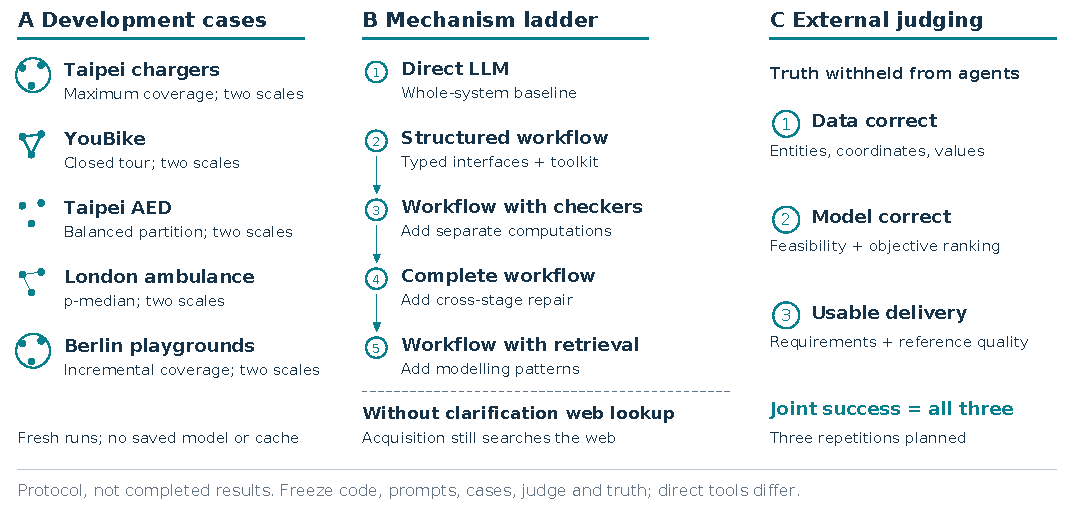
\includegraphics[width=\linewidth]{figures/skill/acceptance-design.pdf}
\caption{Design of the autonomous acceptance comparison, not completed experimental results.
Five development families each have two scales. The ladder identifies the added mechanism in each pipeline configuration; the separate web-lookup arm retains data acquisition.
The direct baseline uses different tools and download limits, so its comparison with the pipeline cannot
isolate agent count. Joint success requires all three acceptance outcomes.}
\label{fig:acceptancedesign}
\end{figure}


\paragraph{External acceptance criteria.}
A deterministic judge reads truth that is never supplied to the runtime agents. \emph{Data:} the instance's
entities must map one-to-one to real entities, by identifier or name first and by coordinates (within a
case-specific tolerance) only for what remains; name-matched entities must still have coordinates near their
own entity and no two entities may share coordinates; measured values must match entity by entity and totals
must equal the official figures. \emph{Model:} with the decision variables fixed to 30 sampled decisions that
satisfy the original request (for selection cases, half of them clustered so that service areas overlap) and
helper variables optimized by MILP, the model must accept every sample and rank them like the independent
metric (Spearman $\geq 0.9$); decisions that break the request must be rejected. \emph{Delivery:} the delivered
solution must satisfy the original request and stay within 10\% of a reference computed on the raw data
(greedy selection, nearest neighbour with 2-opt, greedy grouping with swaps, or the exact optimum). Solutions
from the annealer and from the conventional baseline both count, and are reported separately. A model the judge
cannot read, or cannot compare because the data are wrong, is ``unverifiable'' and counts as incorrect in the
primary analysis. For live feeds, the truth is recomputed from the very official file the run downloaded; runs
that used another source are judged against a pre-downloaded official snapshot and flagged. The judge never
raises: unexpected output becomes a failed or unverifiable gate. Self-tests confirm that correct synthetic
outputs pass and deliberately broken ones fail (dropped entities, copied coordinates, unconverted projected
coordinates, a relaxed cardinality bound, a scattered grouping, a poor tour).

\paragraph{Freezing, preregistration and held-out cases.}
Code, prompts, the modelling-pattern library, solver configuration, case definitions, judge and truth are hashed
before a batch; any change requires a new batch tag. A preflight script must pass before a batch starts (tests,
judge self-tests, a truth and a judge for every case, LLM server, solver reachability, hardware budget, no other
experiment running). Hypotheses, metrics, the treatment of unverifiable models and the rerun rule (only
infrastructure failures) are fixed in advance. The development cases, the modelling-pattern library and the judge
were revised after observing development runs; generalization is therefore assessed on held-out cases defined and
run only after the code is frozen again.

\paragraph{Development observations.}
Development runs used changing code and are not a frozen comparison; they are reported for the failure modes they
revealed, not as rates. Mechanisms behaved as designed in several instances: the toolkit's join flags rejected
a village-name join that would have merged homonymous villages and reduced 456 villages to 32; a schema mismatch
found during data preparation (non-unique village names used as identifiers) was routed back to the Modeling
Agent, repaired, and the run delivered an accepted solution; the data double-check exposed an AED instance with
320 rows instead of 48 places and a fabricated extra station. The LLM-written checkers were also wrong several
times: a Data Checker summed category rows twice, a Requirement Checker computed great-circle distances without
converting degrees to radians, and another invented a fixed start station. The last one made the controller
discard an annealer tour shorter than the reference in favour of a weaker baseline, which motivated two rules:
a late Checker objection does not trigger a repair when no solver call remains to re-solve, and a repaired
version without a solution falls back to the earlier version's annealer result. Other recurring failures were
a modelling-technique (subtour elimination) recorded as a user requirement, an edge-based tour model without a
single-tour guarantee, crowd-sourced points used instead of a named official feed, and report spreadsheets
mistaken for record tables; each led to a problem-independent rule or check described in \cref{sec:system}.
We report no aggregate autonomous success rate or mechanism effect yet.

\section{Limitations and Open Work}
\label{sec:limitations}

We state plainly what the current evidence does and does not support.

\begin{itemize}
  \item \textbf{Real-data acceptance remains limited.} A specified-source UCI red-wine pilot reached a local SA
        solution both through saved-model recovery and a fresh run, with independent case-specific checks.
        Recovered wholesale-customer and real-network cases also delivered independently checked solutions.
        A ten-case real-data acceptance catalog has been prepared but not fully executed. The new autonomous
        batch suite uses Taipei chargers, YouBike routing and AED grouping (\cref{sec:autonomousprotocol});
        it has development smoke tests but no completed frozen repeated comparison. Earlier Paris itinerary
        and labour-law scheduling examples remain prospective. The preprocessing toolkit reproduces official
        totals on real public data, which is narrower evidence than autonomous acquisition and modelling. In one run on real Taipei data, the local Data Adapter produced a valid instance but
        ignored the toolkit, wrote its own transformations and added licence information that was not in the
        sources; the provenance record must therefore be written by code, not by the model.
  \item \textbf{Checker independence is limited.} Separate prompts and computations reduce direct reuse of
        Adapter or model code, but the roles share a base LLM and schema and can share the same error.
        Counts and totals do not establish per-entity data correctness, and sampled requirement checks do not
        verify every feasible state. The external judge remains case-specific and can itself fail.
  \item \textbf{Agent and retrieval effects remain hypotheses.} The direct baseline differs in tools,
        acquisition limits and feedback, so it does not isolate agent count. The new modelling-pattern
        retrieval ablation is implemented but has no completed repeated result. Earlier null results for
        splitting tuning roles or retrieving tuning knowledge do not answer the modelling-stage question.
  \item \textbf{Hardware evidence remains small.} Subsequent CGA and Leap Hybrid BQM comparisons use three repetitions per
        condition. Hybrid service results are distinct from direct QPU sampling, and use a ten-second limit
        versus the three-second CGA ceiling; the resource allocations do not establish hardware superiority.
        Effects depend on the problem; Fujitsu DA rejected a submission due to its monthly
        account limit. The earlier simulation advantage is small, and neither role splitting nor retrieval
        helped there. Large-scale repeated hardware and held-out backend-transfer studies remain open.
  \item \textbf{Functional coverage is not end-to-end reliability.} The integration checks in
        \cref{sec:integrationchecks} exercise parameterized compilation, local search and recovery fixtures.
        They do not establish success rates for live data acquisition, LLM diagnosis or model repair, and the
        new penalty policies have an eight-instance repeated simulation comparison, in which defaults had the
        lowest mean gap, plus small actual-CGA comparisons. A feasible
        baseline gives a comparison point, not a guarantee of application-level quality.
  \item \textbf{Recovery has a limited scope.} Checkpoint resume supports the four history-based penalty
        policies on typed models, not the existing agent or joint Optuna state. Supported searches can resume
        through the UI or command-line tool. An interrupted external solver call may
        require inspection before resubmission. Requirement coverage and formula-change checks cannot prove
        correctness of the original model, and a single-flip penalty floor cannot certify every global
        optimum. Data substitutions and requirement changes still need user judgment.
  \item \textbf{Small local model.} The local model fails as a modeller in recognisable ways (\cref{sec:mechanisms});
        our checks catch structural failures but not every semantic one: a model may pass all checks and still
        replace the requested objective with a weaker surrogate, which only the user's review catches. Data
        interpretation is also fallible (a labour-law rule of two rest days per seven was simplified to one).
  \item \textbf{Scale.} Brute-force verification is limited to about 26 variables; larger encodings are reported
        as unverifiable. Routing on the GPU annealer degrades beyond about 30 stops; multi-vehicle routing
        produced the weakest models of all categories, and connectivity constraints (network design) remain hard
        to express.
  \item \textbf{Benchmark scope.} The 100 benchmarks have tiny instances (median five variables), and our
        12-category suite uses synthetic data. Neither measures real-world difficulty.
  \item \textbf{Non-determinism.} Even at temperature zero, 27\% of benchmark outcomes changed between identical
        runs; all comparisons in this paper therefore use repeated runs for local conditions.
\end{itemize}


\bibliographystyle{plainnat}
\bibliography{references}

\clearpage
\appendix
\section{Reproducibility settings}
\label{app:details}
This appendix records the settings needed to interpret the experiments. Full per-condition tables,
bootstrap intervals, timing audits and development records are retained in the supplementary experiment report.

\paragraph{Frozen-model comparisons.}
Models, data, objectives and original constraints were held fixed before comparing solver policies.
Table~\ref{tab:solverprotocol} gives per-call settings; limits are ceilings and early stopping can reduce actual
calls. External repetitions are new submissions rather than controlled hardware seeds. SA sweeps, CGA search
seconds and Hybrid service seconds are different resources and do not support a hardware-superiority claim.

\begin{table}[h]
\centering\small
\caption{Settings of the frozen-model comparisons.}
\label{tab:solverprotocol}
\begin{tabular}{@{}lp{5.6cm}ll@{}}
\toprule
Comparison & Per-call setting & Call ceiling & Repetitions \\
\midrule
Extended SA penalty & 60 reads, 300 sweeps & 6 & 10 seeds \\
SA backend comparison & 60 reads, 300 sweeps & 3 & 3 \\
CGA backend comparison & 3-second search limit & 3 & 3 \\
Leap Hybrid BQM & Explicit 10-second service limit & 3 & 3 \\
40-station routing, SA & 30 reads, 300 sweeps & 3 & 3 \\
40-station routing, CGA & 3-second search limit & 3 & 3 \\
\bottomrule
\end{tabular}
\end{table}

\paragraph{Statistics and references.}
The extended penalty comparison uses eight instances, eight policies and ten seeds (640 runs). Hierarchical
bootstrap intervals use 10,000 draws, resampling instances and then seeds within instances. Paired Wilcoxon
tests use eight per-instance seed-averaged differences, with Holm correction for the four penalty-policy
comparisons against defaults. Exact references are used for the three small frozen models and the two encoding
instances; the 40-station routing reference is a feasible 20-restart 2-opt tour, not an optimum.

\paragraph{Ancillary solver checks.}
The encoding ablation covers two knapsack instances, three encodings, 60 SA conditions and 18 CGA conditions.
All returned feasible results, but unbalanced encoding missed the 12-item CGA optimum (gap 0.0387).
A separate hand-written 40-station routing model uses 1,600 decision variables; 17 of 18 runs returned feasible
tours, whose mean distances exceeded the 7.695977-km heuristic reference. These checks characterize solving,
not autonomous data preparation or LLM modelling.

\paragraph{Functional validation.}
\label{sec:integrationchecks}
The current offline suite passes 146 tests covering compilation, data interfaces, checker fixtures, bounded
recovery, artifact versions and checkpoint resume. Supported penalty-only policies reproduce uninterrupted
search histories after resume; changed models and unresolved external calls are rejected. Generated-code
execution has process timeouts. These fixture-based checks establish implementation behaviour, not live
acquisition success, LLM semantic correctness or autonomous repair rates.


\end{document}
